% Options for packages loaded elsewhere
\PassOptionsToPackage{unicode}{hyperref}
\PassOptionsToPackage{hyphens}{url}
\PassOptionsToPackage{dvipsnames,svgnames,x11names}{xcolor}
%
\documentclass[
  letterpaper,
  DIV=11,
  numbers=noendperiod]{scrartcl}

\usepackage{amsmath,amssymb}
\usepackage{lmodern}
\usepackage{iftex}
\ifPDFTeX
  \usepackage[T1]{fontenc}
  \usepackage[utf8]{inputenc}
  \usepackage{textcomp} % provide euro and other symbols
\else % if luatex or xetex
  \usepackage{unicode-math}
  \defaultfontfeatures{Scale=MatchLowercase}
  \defaultfontfeatures[\rmfamily]{Ligatures=TeX,Scale=1}
\fi
% Use upquote if available, for straight quotes in verbatim environments
\IfFileExists{upquote.sty}{\usepackage{upquote}}{}
\IfFileExists{microtype.sty}{% use microtype if available
  \usepackage[]{microtype}
  \UseMicrotypeSet[protrusion]{basicmath} % disable protrusion for tt fonts
}{}
\makeatletter
\@ifundefined{KOMAClassName}{% if non-KOMA class
  \IfFileExists{parskip.sty}{%
    \usepackage{parskip}
  }{% else
    \setlength{\parindent}{0pt}
    \setlength{\parskip}{6pt plus 2pt minus 1pt}}
}{% if KOMA class
  \KOMAoptions{parskip=half}}
\makeatother
\usepackage{xcolor}
\setlength{\emergencystretch}{3em} % prevent overfull lines
\setcounter{secnumdepth}{-\maxdimen} % remove section numbering
% Make \paragraph and \subparagraph free-standing
\ifx\paragraph\undefined\else
  \let\oldparagraph\paragraph
  \renewcommand{\paragraph}[1]{\oldparagraph{#1}\mbox{}}
\fi
\ifx\subparagraph\undefined\else
  \let\oldsubparagraph\subparagraph
  \renewcommand{\subparagraph}[1]{\oldsubparagraph{#1}\mbox{}}
\fi


\providecommand{\tightlist}{%
  \setlength{\itemsep}{0pt}\setlength{\parskip}{0pt}}\usepackage{longtable,booktabs,array}
\usepackage{calc} % for calculating minipage widths
% Correct order of tables after \paragraph or \subparagraph
\usepackage{etoolbox}
\makeatletter
\patchcmd\longtable{\par}{\if@noskipsec\mbox{}\fi\par}{}{}
\makeatother
% Allow footnotes in longtable head/foot
\IfFileExists{footnotehyper.sty}{\usepackage{footnotehyper}}{\usepackage{footnote}}
\makesavenoteenv{longtable}
\usepackage{graphicx}
\makeatletter
\def\maxwidth{\ifdim\Gin@nat@width>\linewidth\linewidth\else\Gin@nat@width\fi}
\def\maxheight{\ifdim\Gin@nat@height>\textheight\textheight\else\Gin@nat@height\fi}
\makeatother
% Scale images if necessary, so that they will not overflow the page
% margins by default, and it is still possible to overwrite the defaults
% using explicit options in \includegraphics[width, height, ...]{}
\setkeys{Gin}{width=\maxwidth,height=\maxheight,keepaspectratio}
% Set default figure placement to htbp
\makeatletter
\def\fps@figure{htbp}
\makeatother

\KOMAoption{captions}{tableheading}
\makeatletter
\makeatother
\makeatletter
\makeatother
\makeatletter
\@ifpackageloaded{caption}{}{\usepackage{caption}}
\AtBeginDocument{%
\ifdefined\contentsname
  \renewcommand*\contentsname{Table of contents}
\else
  \newcommand\contentsname{Table of contents}
\fi
\ifdefined\listfigurename
  \renewcommand*\listfigurename{List of Figures}
\else
  \newcommand\listfigurename{List of Figures}
\fi
\ifdefined\listtablename
  \renewcommand*\listtablename{List of Tables}
\else
  \newcommand\listtablename{List of Tables}
\fi
\ifdefined\figurename
  \renewcommand*\figurename{Figure}
\else
  \newcommand\figurename{Figure}
\fi
\ifdefined\tablename
  \renewcommand*\tablename{Table}
\else
  \newcommand\tablename{Table}
\fi
}
\@ifpackageloaded{float}{}{\usepackage{float}}
\floatstyle{ruled}
\@ifundefined{c@chapter}{\newfloat{codelisting}{h}{lop}}{\newfloat{codelisting}{h}{lop}[chapter]}
\floatname{codelisting}{Listing}
\newcommand*\listoflistings{\listof{codelisting}{List of Listings}}
\makeatother
\makeatletter
\@ifpackageloaded{caption}{}{\usepackage{caption}}
\@ifpackageloaded{subcaption}{}{\usepackage{subcaption}}
\makeatother
\makeatletter
\@ifpackageloaded{tcolorbox}{}{\usepackage[many]{tcolorbox}}
\makeatother
\makeatletter
\@ifundefined{shadecolor}{\definecolor{shadecolor}{rgb}{.97, .97, .97}}
\makeatother
\makeatletter
\makeatother
\ifLuaTeX
  \usepackage{selnolig}  % disable illegal ligatures
\fi
\IfFileExists{bookmark.sty}{\usepackage{bookmark}}{\usepackage{hyperref}}
\IfFileExists{xurl.sty}{\usepackage{xurl}}{} % add URL line breaks if available
\urlstyle{same} % disable monospaced font for URLs
\hypersetup{
  pdftitle={AN ANALYSIS OF PORTUGUESE BANK MARKETING DATA},
  pdfauthor={TEAM 11: Anjali Mudgal, Guoshan Yu, Medhasweta Sen},
  colorlinks=true,
  linkcolor={blue},
  filecolor={Maroon},
  citecolor={Blue},
  urlcolor={Blue},
  pdfcreator={LaTeX via pandoc}}

\title{AN ANALYSIS OF PORTUGUESE BANK MARKETING DATA}
\usepackage{etoolbox}
\makeatletter
\providecommand{\subtitle}[1]{% add subtitle to \maketitle
  \apptocmd{\@title}{\par {\large #1 \par}}{}{}
}
\makeatother
\subtitle{The George Washington University (DATS 6103: An Introduction
to Data Mining)}
\author{TEAM 11: Anjali Mudgal, Guoshan Yu, Medhasweta Sen}
\date{December 20, 2022}

\begin{document}
\maketitle
\ifdefined\Shaded\renewenvironment{Shaded}{\begin{tcolorbox}[breakable, frame hidden, enhanced, boxrule=0pt, borderline west={3pt}{0pt}{shadecolor}, sharp corners, interior hidden]}{\end{tcolorbox}}\fi

\hypertarget{introduction}{%
\section{INTRODUCTION}\label{introduction}}

Bank marketing is the practice of attracting and acquiring new customers
through traditional media and digital media strategies. The use of these
media strategies helps determine what kind of customer is attracted to a
certain institutions. This also includes different banking institutions
purposefully using different strategies to attract the type of customer
they want to do business with.

Marketing has evolved from a communication role to a revenue generating
role. The consumer has evolved from being a passive recipient of
marketing messages to an active participant in the marketing process.
Technology has evolved from being a means of communication to a means of
data collection and analysis. Data analytics has evolved from being a
means of understanding the consumer to a means of understanding the
consumer and the institution.

Bank marketing strategy is increasingly focused on digital channels,
including social media, video, search and connected TV. As bank and
credit union marketers strive to promote brand awareness, they need a
new way to assess channel ROI and more accurate data to enable
personalized offers. Add to that the growing importance of
purpose-driven marketing.

The relentless pace of digitization is disrupting not only the
established order in banking, but bank marketing strategies. Marketers
at both traditional institutions and digital disruptors are feeling the
pressure.

Just as bank marketers begin to master one channel, consumers move to
another. Many now toggle between devices on a seemingly infinite number
of platforms, making it harder than ever for marketers to pin down the
right consumers at the right time in the right place.

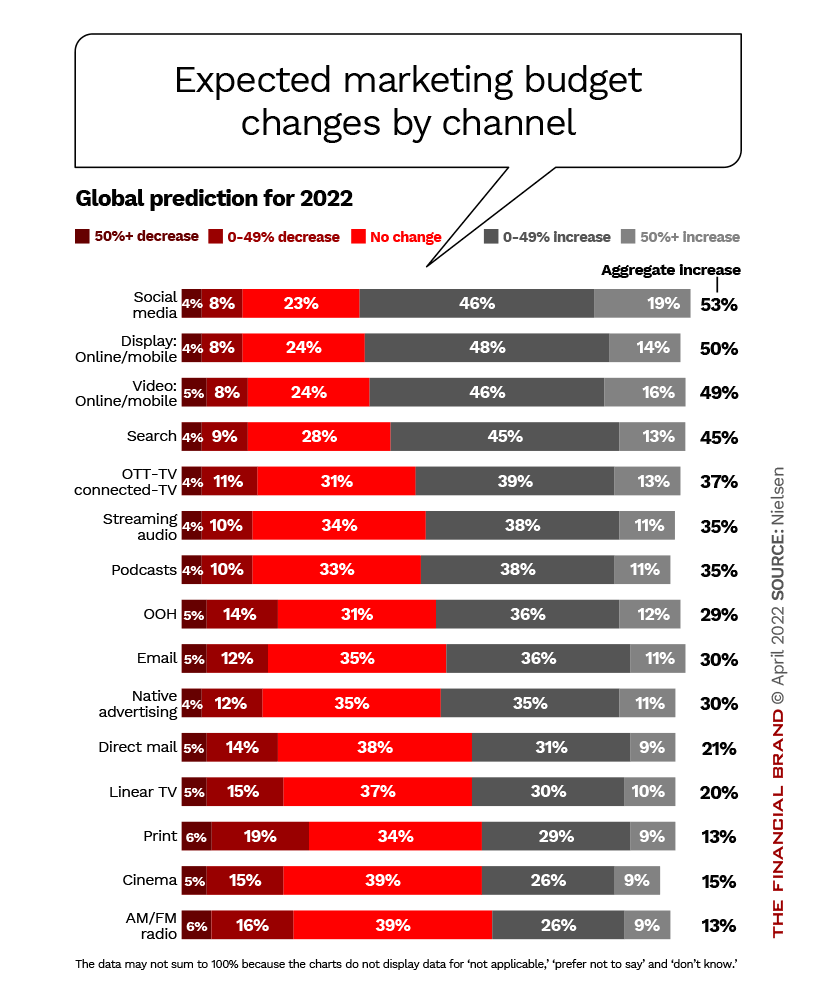
\includegraphics{expected-marketing-budget-changes-by-channel.png}

\hypertarget{the-data-set}{%
\subsection{The Data Set}\label{the-data-set}}

The data set used in this analysis is from a Portuguese bank. The data
set contains 41,188 observations and 21 variables. The variables include
the following:

\begin{enumerate}
\def\labelenumi{\arabic{enumi}.}
\item
  \begin{itemize}
  \tightlist
  \item
    age (numeric)
  \end{itemize}
\item
  \begin{itemize}
  \tightlist
  \item
    job : type of job (categorical:
    `admin.',`blue-collar',`entrepreneur',`housemaid',`management',`retired',`self-employed',`services',`student',`technician',`unemployed',`unknown')
  \end{itemize}
\item
  \begin{itemize}
  \tightlist
  \item
    marital : marital status (categorical:
    `divorced',`married',`single',`unknown'; note: `divorced' means
    divorced or widowed)
  \end{itemize}
\item
  \begin{itemize}
  \tightlist
  \item
    education (categorical:
    `basic.4y',`basic.6y',`basic.9y',`high.school',`illiterate',`professional.course',`university.degree',`unknown')
  \end{itemize}
\item
  \begin{itemize}
  \tightlist
  \item
    default: has credit in default? (categorical: `no',`yes',`unknown')
  \end{itemize}
\item
  \begin{itemize}
  \tightlist
  \item
    housing: has housing loan? (categorical: `no',`yes',`unknown')
  \end{itemize}
\item
  \begin{itemize}
  \tightlist
  \item
    loan: has personal loan? (categorical: `no',`yes',`unknown')
  \end{itemize}
\item
  \begin{itemize}
  \tightlist
  \item
    contact: contact communication type (categorical:
    `cellular',`telephone')
  \end{itemize}
\item
  \begin{itemize}
  \tightlist
  \item
    month: last contact month of year (categorical: `jan', `feb', `mar',
    \ldots, `nov', `dec')
  \end{itemize}
\item
  \begin{itemize}
  \tightlist
  \item
    day\_of\_week: last contact day of the week (categorical:
    `mon',`tue',`wed',`thu',`fri')
  \end{itemize}
\item
  \begin{itemize}
  \tightlist
  \item
    duration: last contact duration, in seconds (numeric). Important
    note: this attribute highly affects the output target (e.g., if
    duration=0 then y=`no'). Yet, the duration is not known before a
    call is performed. Also, after the end of the call y is obviously
    known. Thus, this input should only be included for benchmark
    purposes and should be discarded if the intention is to have a
    realistic predictive model.
  \end{itemize}
\item
  \begin{itemize}
  \tightlist
  \item
    campaign: number of contacts performed during this campaign and for
    this client (numeric, includes last contact)
  \end{itemize}
\item
  \begin{itemize}
  \tightlist
  \item
    pdays: number of days that passed by after the client was last
    contacted from a previous campaign (numeric; 999 means client was
    not previously contacted)
  \end{itemize}
\item
  \begin{itemize}
  \tightlist
  \item
    previous: number of contacts performed before this campaign and for
    this client (numeric)
  \end{itemize}
\item
  \begin{itemize}
  \tightlist
  \item
    poutcome: outcome of the previous marketing campaign (categorical:
    `failure',`nonexistent',`success')
  \end{itemize}
\item
  \begin{itemize}
  \tightlist
  \item
    emp.var.rate: employment variation rate - quarterly indicator
    (numeric)
  \end{itemize}
\item
  \begin{itemize}
  \tightlist
  \item
    cons.price.idx: consumer price index - monthly indicator (numeric)
  \end{itemize}
\item
  \begin{itemize}
  \tightlist
  \item
    cons.conf.idx: consumer confidence index - monthly indicator
    (numeric)
  \end{itemize}
\item
  \begin{itemize}
  \tightlist
  \item
    euribor3m: euribor 3 month rate - daily indicator (numeric)
  \end{itemize}
\item
  \begin{itemize}
  \tightlist
  \item
    nr.employed: number of employees - quarterly indicator (numeric)
  \end{itemize}
\item
  \begin{itemize}
  \tightlist
  \item
    balance - average yearly balance, in euros (numeric)
  \end{itemize}
\item
  \begin{itemize}
  \tightlist
  \item
    y - has the client subscribed a term deposit? (binary: `yes',`no')
  \end{itemize}
\end{enumerate}

\hypertarget{the-smart-questions}{%
\subsection{The SMART Questions}\label{the-smart-questions}}

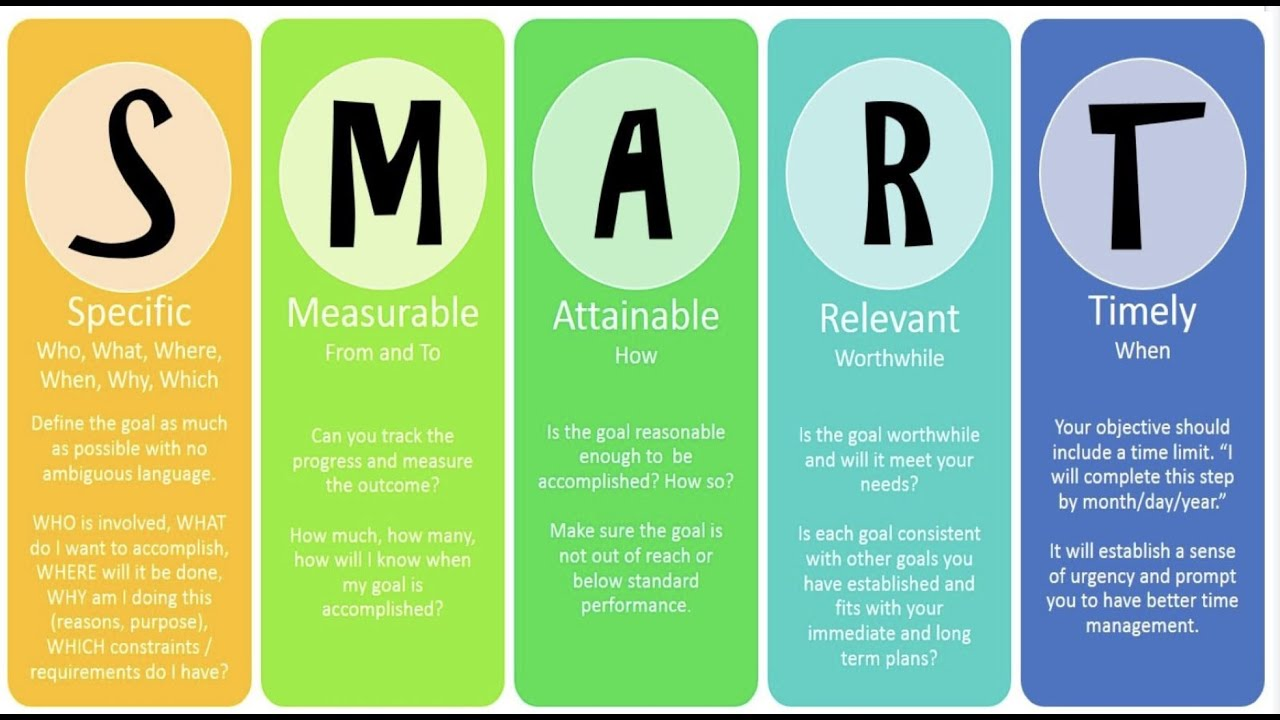
\includegraphics{maxresdefault.jpg} The SMART questions are as follows:

1.Relationship between subscribing the term deposit and how much the
customer is contacted (last contact, Campaign, Pdays, Previous Number of
contacts)

\begin{enumerate}
\def\labelenumi{\arabic{enumi}.}
\setcounter{enumi}{1}
\tightlist
\item
  Find out the financially stable population? Will that affect the
  outcome?
\end{enumerate}

3.Effect of dimensionality reduction on accuracy of the model.

\begin{enumerate}
\def\labelenumi{\arabic{enumi}.}
\setcounter{enumi}{3}
\tightlist
\item
  How are the likelihood of subscriptions affected by social and
  economic factors?
\end{enumerate}

Throughout the paper we would try to answer the questions

Importing the required libraries

\hypertarget{importing-the-dataset}{%
\subsection{Importing the dataset}\label{importing-the-dataset}}

\hypertarget{basic-information-about-the-data}{%
\subsection{Basic Information about the
data}\label{basic-information-about-the-data}}

\begin{verbatim}
Shape of dataset is : (45211, 23)
<class 'pandas.core.frame.DataFrame'>
RangeIndex: 45211 entries, 0 to 45210
Data columns (total 23 columns):
 #   Column          Non-Null Count  Dtype  
---  ------          --------------  -----  
 0   age             45211 non-null  int64  
 1   job             45211 non-null  object 
 2   marital         45211 non-null  object 
 3   education       45211 non-null  object 
 4   default         45211 non-null  object 
 5   balance         45211 non-null  int64  
 6   housing         45211 non-null  object 
 7   loan            45211 non-null  object 
 8   contact         45211 non-null  object 
 9   day             45211 non-null  int64  
 10  month           45211 non-null  object 
 11  duration        45211 non-null  int64  
 12  campaign        45211 non-null  int64  
 13  pdays           45211 non-null  int64  
 14  previous        45211 non-null  int64  
 15  poutcome        45211 non-null  object 
 16  y               45211 non-null  int64  
 17  month_int       45211 non-null  int64  
 18  cons.conf.idx   45211 non-null  float64
 19  emp.var.rate    45211 non-null  float64
 20  euribor3m       45211 non-null  float64
 21  nr.employed     45211 non-null  float64
 22  cons.price.idx  45211 non-null  float64
dtypes: float64(5), int64(9), object(9)
memory usage: 7.9+ MB
Columns in dataset 
 None
\end{verbatim}

\hypertarget{exploratory-data-analysis-eda}{%
\section{Exploratory Data Analysis
(EDA)}\label{exploratory-data-analysis-eda}}

\hypertarget{distribution-of-ytarget-variable}{%
\subsection{Distribution of y(target)
variable}\label{distribution-of-ytarget-variable}}

\includegraphics{Summary_files/figure-pdf/cell-7-output-1.pdf}

We have 45,211 datapoints, if our model predicts only 0 as output, we
would still get 88\% accuracy, so our dataset is unbalanced which may
gives misleading results. Along with the accuracy, we will also consider
precision and recall for evaluation.

\hypertarget{missing-values-and-outliers}{%
\subsection{Missing values and
Outliers}\label{missing-values-and-outliers}}

\hypertarget{education}{%
\subsubsection{Education}\label{education}}

Here, even though we do not have any missing values but we have
`unknown' and `other' as categories, so we will first get rid of them.
The variables with `unknown' rows are Education and Contact showned
below.

\begin{verbatim}
Text(0.5, 1.0, 'Type of education Distribution')
\end{verbatim}

\includegraphics{Summary_files/figure-pdf/cell-8-output-2.pdf}

\hypertarget{contact}{%
\subsubsection{Contact}\label{contact}}

\begin{verbatim}
Text(0.5, 1.0, 'Type of Contact Distribution')
\end{verbatim}

\includegraphics{Summary_files/figure-pdf/cell-9-output-2.pdf}

\begin{itemize}
\tightlist
\item
  since the type of communication(cellular and telephone) is not really
  a good indicator of subcription, we drop this variable.
\end{itemize}

\hypertarget{poutcome}{%
\subsubsection{Poutcome}\label{poutcome}}

\includegraphics{Summary_files/figure-pdf/cell-10-output-1.pdf}

\begin{tabular}{lr}
\toprule
{} &      0 \\
poutcome &        \\
\midrule
failure  &   4901 \\
other    &   1840 \\
success  &   1511 \\
unknown  &  36959 \\
\bottomrule
\end{tabular}

There are \emph{36959 unknown} values(82\%) and 1840 values with
other(4.07\% ) category, we will directly drop these columns.

\hypertarget{outliers}{%
\subsection{Outliers}\label{outliers}}

\includegraphics{Summary_files/figure-pdf/cell-11-output-1.pdf}

\begin{itemize}
\tightlist
\item
  There are outliers in duration and balance so we need to get rid of
  them.
\end{itemize}

\hypertarget{data-cleaning}{%
\section{Data Cleaning}\label{data-cleaning}}

\begin{itemize}
\tightlist
\item
  Contact is not useful so we drop it.
\item
  In poutcome, we have a lot of `unknown' and `other' values so we drop
  it.\\
\item
  Day is not giving any relevant infomation so we drop it.
\item
  Removing the unknowns from `job' and `education' columns.
\item
  Remove the outliers from balance and duration.
\end{itemize}

\hypertarget{dropping-the-irrelavant-columns-and-missing-values}{%
\subsection{Dropping the irrelavant columns and missing
values}\label{dropping-the-irrelavant-columns-and-missing-values}}

\begin{verbatim}
for job
unknown : 288
dropping rows with value as unknown in job
for education
unknown : 1730
dropping rows with value as unknown in education
\end{verbatim}

\hypertarget{outlier-removal}{%
\subsection{Outlier removal}\label{outlier-removal}}

We have outliers in balance and duration, so to get rid of them we would
try to remove the enteries few standard deviation away, since from the
histograms most of the enteries are around mean only, we are removing
the enteries more than 3SD away.

\hypertarget{balance---outliers}{%
\subsubsection{\texorpdfstring{\emph{Balance -
Outliers}}{Balance - Outliers}}\label{balance---outliers}}

\begin{verbatim}
removing entries before balance   -7772.283533
dtype: float64 and after balance    10480.338218
dtype: float64
\end{verbatim}

\hypertarget{duration---outliers}{%
\subsubsection{\texorpdfstring{\emph{Duration -
Outliers}}{Duration - Outliers}}\label{duration---outliers}}

Dropping rows where the duration of calls is less than 5sec since that
is irrelevant. And also since converting the call duration in minutes
rather than seconds makes more sense we would convert it into minutes.

plotting violen plot for duration and balance after cleaning data

\includegraphics{Summary_files/figure-pdf/cell-15-output-1.pdf}

\hypertarget{data-visualization}{%
\section{Data Visualization}\label{data-visualization}}

Let' visualize important relationships between variables now.

\hypertarget{smart-question-1}{%
\subsection{SMART Question 1 :}\label{smart-question-1}}

Relationship between subscribing the term deposit and how much the
customer is contacted (last contact, Campaign, Pdays, Previous Number of
contacts)

Answer : Based on last contact info only number of contacts performed
during this campaign is contributing a lot towards subscription rates.

Suggestion: People who are contacted less than 5 times should be
targeted more. Also, they could contact in less frequency in order to
attract more target customers. The plot below shows the relationship
between the number of calls and duration vs subscription

\hypertarget{number-of-calls-versus-duration-and-affect-on-subscription}{%
\subsubsection{Number of calls versus Duration and affect on
subscription}\label{number-of-calls-versus-duration-and-affect-on-subscription}}

Here if we notice, people are more likely to subscribe if the number of
calls are less than 5.

\includegraphics{Summary_files/figure-pdf/cell-16-output-1.pdf}

Checking between pdays and previous as well

Here as we can see from the t- test, t

\begin{enumerate}
\def\labelenumi{\arabic{enumi}.}
\setcounter{enumi}{12}
\item
  \begin{itemize}
  \tightlist
  \item
    pdays: number of days that passed by after the client was last
    contacted from a previous campaign (numeric; 999 means client was
    not previously contacted)
  \end{itemize}
\item
  \begin{itemize}
  \tightlist
  \item
    previous: number of contacts performed before this campaign and for
    this client (numeric)
  \end{itemize}
\end{enumerate}

We can notice from the plot that there is no relationship between
subscription with pdays or previous. The datapoints are distrubuted
randomly along the axies.

\includegraphics{Summary_files/figure-pdf/cell-17-output-1.pdf}

\hypertarget{month-wise-subscription}{%
\subsection{Month wise subscription}\label{month-wise-subscription}}

\begin{verbatim}
Text(0.5, 0, 'Month')
\end{verbatim}

\includegraphics{Summary_files/figure-pdf/cell-18-output-2.pdf}

Maximum percentage of people have subscribed in the month of March but
bank is contacting people more in the month of May.

\textbf{Suggestion}:So it's better to contact customer's based on the
subcription rate plot.

\hypertarget{smart-question-7-how-are-the-likelihood-of-subscriptions-affected-by-social-and-economic-factors}{%
\subsubsection{SMART Question 7: How are the likelihood of subscriptions
affected by social and economic
factors?}\label{smart-question-7-how-are-the-likelihood-of-subscriptions-affected-by-social-and-economic-factors}}

\begin{verbatim}
   month  cons.conf.idx  emp.var.rate  euribor3m  nr.employed
0    jan           1310          1310       1310         1310
1    feb           2492          2492       2492         2492
2    mar            439           439        439          439
3    apr           2772          2772       2772         2772
4    may          13050         13050      13050        13050
5    jun           4874          4874       4874         4874
6    jul           6550          6550       6550         6550
7    aug           5924          5924       5924         5924
8    sep            514           514        514          514
9    oct            661           661        661          661
10   nov           3679          3679       3679         3679
11   dec            195           195        195          195
\end{verbatim}

\textbf{Answer} : Based on the above table we can see that there is no
distinguishable difference in the month of march or may from rest of all
the month, so social and economic factor \textbf{do not have major
influence} on the outcome.

\hypertarget{smart-question-2}{%
\subsubsection{SMART Question 2}\label{smart-question-2}}

Find out the \textbf{financially stable} population? Will that affect
the outcome?

We will try to find the financially stable population based on age,
jobs, loan and balance.

\hypertarget{loan}{%
\subsubsection{Loan}\label{loan}}

\begin{verbatim}
Text(0.5, 1.0, 'Type of loan Distribution')
\end{verbatim}

\includegraphics{Summary_files/figure-pdf/cell-21-output-2.pdf}

\begin{verbatim}
Text(0.5, 1.0, 'Type of housing Distribution')
\end{verbatim}

\includegraphics{Summary_files/figure-pdf/cell-22-output-2.pdf}

People with housing loans are less likely to subscribe to term deposit
but the difference here is not huge.

\begin{verbatim}
Text(0.5, 1.0, 'Type of default Distribution')
\end{verbatim}

\includegraphics{Summary_files/figure-pdf/cell-23-output-2.pdf}

So people who have not paid back there loans and have credits, have not
subcribed to the term deposit.

\begin{itemize}
\tightlist
\item
  people who have loans are subscribing to term deposit less.
\end{itemize}

\hypertarget{age}{%
\subsubsection{Age}\label{age}}

Elder people might be more financially stable since they are subscriped
to the term deposit more.

\includegraphics{Summary_files/figure-pdf/cell-24-output-1.pdf}

\begin{itemize}
\tightlist
\item
  People who are old are more likely to subscribe to term deposit.
\end{itemize}

\hypertarget{job}{%
\subsubsection{Job}\label{job}}

\includegraphics{Summary_files/figure-pdf/cell-25-output-1.pdf}

\includegraphics{Summary_files/figure-pdf/cell-25-output-2.pdf}

People in blue collar and management jobs are contacted more, which
should not be the case. Since they have less subscription rates. Unlike
popular assumption, students, retired and unemployment seem to have a
high subscription rates. Even though they are contacted very less.

\textbf{suggestion}: The high subscripted rate group(students, retired
and unemployment) should be contacted more.

\hypertarget{balance}{%
\subsubsection{Balance}\label{balance}}

Checking the subscriptions in each balance groups

\begin{verbatim}
           balGroup  % Contacted  % Subscription
0       low balance    60.339143       10.503513
1  moderate balance    17.399906       14.036275
2      high balance    13.709374       16.715341
3          Negative     8.551578        5.700909
       balanceGroup Contact Rate Subscription Rate
0          Negative     8.551578          5.700909
1       low balance    60.339143         10.503513
2  moderate balance    17.399906         14.036275
3      high balance    13.709374         16.715341
\end{verbatim}

\includegraphics{Summary_files/figure-pdf/cell-26-output-2.pdf}

\textbf{suggestion}:People with moderate to high balance, are contacted
less but they have high subscription rates so bank should target them
more.

It might be possible that balance group and jobs are telling the same
information since some jobs might have high salary and thus balance
groups might be depicting jobs only, so we will try to look at them
together.

Balance Group versus Job

\begin{verbatim}
Text(0.5, 1.0, 'Contact for each balance group in job category')
\end{verbatim}

\includegraphics{Summary_files/figure-pdf/cell-27-output-2.pdf}

\includegraphics{Summary_files/figure-pdf/cell-27-output-3.pdf}

Student and Retired are more likely to subscribe and usually have
moderate to high balance.

We found from the second bar chart that only the low balance groups are
targeted in each category even though moderate to high balance category
are more likely to subscribe.

\hypertarget{data-encoding}{%
\section{Data Encoding}\label{data-encoding}}

\hypertarget{one-hot-encoding}{%
\subsection{One Hot Encoding}\label{one-hot-encoding}}

We would encode `housing',`loan',`default',`job',`education' and
`marital' as they are all categorical variables.

\hypertarget{sin---cos-encoding}{%
\subsection{Sin - Cos encoding}\label{sin---cos-encoding}}

Transforming month into sin and cos so that there cyclic nature (jan-dec
are as close as jan-feb) is retained which is usually lost in label
encoding. Unlike one hot encoding, the dimension will reduce from
12(month\_jan, month\_feb \ldots{} month\_dec) to 2(sin\_month ,
cos\_month)

\begin{verbatim}
<AxesSubplot: xlabel='sin_month', ylabel='cos_month'>
\end{verbatim}

\includegraphics{Summary_files/figure-pdf/cell-30-output-2.pdf}

\hypertarget{dropping-unnecessary-columns-irrelevant-for-modelling}{%
\subsection{Dropping unnecessary columns irrelevant for
modelling}\label{dropping-unnecessary-columns-irrelevant-for-modelling}}

Here we dropped the `month' column as they are encoded. Also, we dropped
irrelvant variables `pdays' and enconomic factors(`cons.conf.idx',
`emp.var.rate', `euribor3m', `nr.employed',`cons.price.idx') for
modelling.

\hypertarget{data-modeling}{%
\section{Data Modeling}\label{data-modeling}}

\hypertarget{splitting-our-dataset}{%
\subsection{Splitting our Dataset}\label{splitting-our-dataset}}

We are splitting our dataset in 1:4 ratio for training and testing set.

\hypertarget{balancing-our-dataset}{%
\subsection{Balancing Our Dataset}\label{balancing-our-dataset}}

We tried to balance our dataset using following methods:

\begin{itemize}
\tightlist
\item
  Upsampling using SMOTE
\item
  Sin and cos transformation from month\_int.
\end{itemize}

\hypertarget{scaling-numeric-variables}{%
\section{Scaling numeric variables}\label{scaling-numeric-variables}}

Scaling age, balance, duration so that our algorithms perform better and
all variables are treated equally. Since all three variables are in
different scales, so we transform them into same standard.

\hypertarget{logistic-regression}{%
\section{Logistic Regression}\label{logistic-regression}}

Performing Logistic Regression on both balanced and unbalanced dataset.
RFE is used in selecting the most important features \#\# Unbalanced
Dataset

\begin{verbatim}
Columns selected by RE ['duration', 'euribor3m', 'cons.price.idx', 'job_blue-collar', 'job_retired', 'job_student', 'education_primary', 'education_tertiary', 'marital_single', 'housing_no', 'housing_yes', 'loan_no', 'loan_yes', 'poutcome_failure', 'poutcome_success', 'month_apr', 'month_aug', 'month_feb', 'month_jan', 'month_jul', 'month_jun', 'month_mar', 'month_nov', 'month_oct', 'age', 'balance']
\end{verbatim}

As we can see from RFE, the most relevant features are :

\begin{itemize}
\tightlist
\item
  Duration
\item
  Housing
\item
  Loan
\item
  Job
\item
  Education
\item
  cos\_month
\end{itemize}

From other features selection techniques and EDA, we can see that `age'
and `balance' also contrubuted to the subscrption, so we added up these
variables as well.

Applying model with selected features

\begin{verbatim}
Accuracy for training set 0.8717311715481172
Accuracy for testing set 0.8713389121338913
Confusion matrix 
[[4759  148]
 [ 590  239]]
              precision    recall  f1-score   support

           0       0.89      0.97      0.93      4907
           1       0.62      0.29      0.39       829

    accuracy                           0.87      5736
   macro avg       0.75      0.63      0.66      5736
weighted avg       0.85      0.87      0.85      5736
\end{verbatim}

Here, the accuracy is 89\% but the precision(0.59) and recall rate
value(0.20) is low. And we also check on the balanced dataset since the
low recall rate might be caused because of the less number of y = 1
value.

\hypertarget{balanced-dataset}{%
\section{Balanced Dataset}\label{balanced-dataset}}

\begin{verbatim}
Columns selected by RE ['duration', 'cons.price.idx', 'job_admin.', 'job_blue-collar', 'job_management', 'job_self-employed', 'job_services', 'job_technician', 'job_unemployed', 'education_primary', 'education_secondary', 'education_tertiary', 'marital_divorced', 'marital_married', 'marital_single', 'housing_no', 'housing_yes', 'loan_yes', 'poutcome_failure', 'month_apr', 'month_aug', 'month_jul', 'month_may', 'month_nov']
\end{verbatim}

\begin{verbatim}
Accuracy for training set 0.9064744536702155
Accuracy for testing set 0.8516387726638772
Confusion matrix 
[[4440  467]
 [ 384  445]]
              precision    recall  f1-score   support

           0       0.92      0.90      0.91      4907
           1       0.49      0.54      0.51       829

    accuracy                           0.85      5736
   macro avg       0.70      0.72      0.71      5736
weighted avg       0.86      0.85      0.85      5736
\end{verbatim}

Here, important features are * Housing * Loan * Job * Education *
Marital Status

We also added the important features from unbalaced dataset * Duration *
Age * Month * Balance

Here even though the precision and recall have improved, and accuracy
has dropped down, but the important relationships are lost since the
training data now is artificially generated datapoints. We will try to
find the optimal cut-off value for original dataset and compare it with
the model for balanced data.

\hypertarget{deciding-cut-off-value-for-logistic-regression---unbalance}{%
\subsubsection{Deciding cut off value for logistic regression -
Unbalance}\label{deciding-cut-off-value-for-logistic-regression---unbalance}}

But to have good values for cut-off we would try to find a cutoff where
the precision and recall values are decent

\begin{verbatim}

Based on plot we would choose 0.25 as cut off 
Accuracy for testing set 0.8589609483960948
Confusion matrix 
[[4447  460]
 [ 349  480]]
              precision    recall  f1-score   support

           0       0.93      0.91      0.92      4907
           1       0.51      0.58      0.54       829

    accuracy                           0.86      5736
   macro avg       0.72      0.74      0.73      5736
weighted avg       0.87      0.86      0.86      5736
\end{verbatim}

\begin{figure}

{\centering \includegraphics{Summary_files/figure-pdf/cell-41-output-2.pdf}

}

\caption{Optimal Cutoff at 0.25}

\end{figure}

Here as after applying feature selection, finding optimized cut-off, we
are able to achieve higher accuracy with optimal precision and recall.
Resulting from the comparison, we would continue our modellings with
unbalance dataset.

\hypertarget{smart-question-5-the-optimal-cut-off-value-for-classification-of-our-imbalance-dataset.}{%
\subsubsection{Smart Question 5: The optimal cut off value for
classification of our imbalance
dataset.}\label{smart-question-5-the-optimal-cut-off-value-for-classification-of-our-imbalance-dataset.}}

\textbf{Answer}: The optimal cut off value for our imbalance dataset is
0.25 as the precision- recall chart indicated.

\hypertarget{smart-question-2-since-the-dataset-is-imbalanced-will-down-samplingup-sampling-or-other-techniques-improve-upon-the-accuracy-of-models.}{%
\subsubsection{SMART Question 2: Since the dataset is imbalanced, will
down sampling/up sampling or other techniques improve upon the accuracy
of
models.}\label{smart-question-2-since-the-dataset-is-imbalanced-will-down-samplingup-sampling-or-other-techniques-improve-upon-the-accuracy-of-models.}}

\textbf{Answer}: As observed from above there is a slight improvement in
accuracy, precision and recall after we apply SMOTE, but that
improvement can also be acheived by adjusting the cut off value as well.
So, we should always try adjusting cut-off first, before upsampling.

For ROC - AUC curve refer (Figure~\ref{fig-roc-curve}).\\
For precision recall curve refer(Figure~\ref{fig-pr-curve}).

\hypertarget{decision-tree}{%
\section{Decision Tree}\label{decision-tree}}

\hypertarget{feature-selection}{%
\subsection{Feature Selection}\label{feature-selection}}

\begin{verbatim}
Feature 0 variable age score 0.09
Feature 1 variable balance score 0.10
Feature 2 variable day score 0.09
Feature 3 variable duration score 0.28
Feature 4 variable campaign score 0.03
Feature 5 variable pdays score 0.06
Feature 6 variable previous score 0.01
Feature 7 variable cons.conf.idx score 0.02
Feature 8 variable emp.var.rate score 0.03
Feature 9 variable euribor3m score 0.02
Feature 11 variable cons.price.idx score 0.02
Feature 29 variable housing_no score 0.02
Feature 30 variable housing_yes score 0.01
Feature 36 variable poutcome_success score 0.06
Feature 43 variable month_jun score 0.01
Important features from decision treee are : 
['age', 'balance', 'day', 'duration', 'campaign', 'pdays', 'previous', 'cons.conf.idx', 'emp.var.rate', 'euribor3m', 'cons.price.idx', 'housing_no', 'housing_yes', 'poutcome_success', 'month_jun']
\end{verbatim}

\includegraphics{Summary_files/figure-pdf/cell-42-output-2.pdf}

Features selected from this algorithm are

\begin{itemize}
\tightlist
\item
  Age
\item
  Balance
\item
  Duration
\item
  Campaign
\item
  Previous
\item
  Housing
\item
  Job
\item
  Education
\item
  Marital
\item
  Month - Sin,cos
\end{itemize}

We have all the important features from EDA here

\hypertarget{hyperparameter-tuning}{%
\subsection{Hyperparameter tuning}\label{hyperparameter-tuning}}

For tuning the hyperparameter's we will use GridSearch CV.

\begin{verbatim}
Fitting 5 folds for each of 168 candidates, totalling 840 fits
\end{verbatim}

\begin{verbatim}
Best parameters from Grid Search CV : 
{'criterion': 'gini', 'max_depth': 6, 'max_features': 0.8, 'splitter': 'best'}
\end{verbatim}

Training model based on the parameters we got from Grid SearchCV.

\begin{verbatim}
0.879881450488145
[[4641  266]
 [ 423  406]]
              precision    recall  f1-score   support

           0       0.92      0.95      0.93      4907
           1       0.60      0.49      0.54       829

    accuracy                           0.88      5736
   macro avg       0.76      0.72      0.74      5736
weighted avg       0.87      0.88      0.87      5736
\end{verbatim}

From the decision tree we have better precision, recall, accuracy and
thus better f1 score. Hence, decision tree is performing better than
logistic regression.

AUC Curve : Figure~\ref{fig-roc-curve}\\
Precision Recall Curve : Figure~\ref{fig-pr-curve}

\hypertarget{random-forest}{%
\section{Random Forest}\label{random-forest}}

\hypertarget{feature-selection-1}{%
\subsection{Feature Selection}\label{feature-selection-1}}

\begin{verbatim}
Important features from random forest :
['age', 'balance', 'day', 'duration', 'campaign', 'pdays', 'previous', 'cons.conf.idx', 'emp.var.rate', 'euribor3m', 'nr.employed', 'cons.price.idx', 'job_management', 'job_technician', 'education_secondary', 'education_tertiary', 'marital_married', 'marital_single', 'housing_no', 'housing_yes', 'poutcome_failure', 'poutcome_success']
\end{verbatim}

\includegraphics{Summary_files/figure-pdf/cell-45-output-2.pdf}

\hypertarget{hyperparameter-tuning-1}{%
\subsection{Hyperparameter Tuning}\label{hyperparameter-tuning-1}}

\begin{verbatim}
Fitting 3 folds for each of 32 candidates, totalling 96 fits
\end{verbatim}

\begin{verbatim}
{'bootstrap': True, 'max_depth': 100, 'max_features': 3, 'n_estimators': 1000}
\end{verbatim}

\begin{verbatim}
Training accuracy 1.0
Testing set accuracy 0.8865062761506276
[[4714  193]
 [ 458  371]]
              precision    recall  f1-score   support

           0       0.91      0.96      0.94      4907
           1       0.66      0.45      0.53       829

    accuracy                           0.89      5736
   macro avg       0.78      0.70      0.73      5736
weighted avg       0.87      0.89      0.88      5736
\end{verbatim}

We are getting best performance from Random Forest but we are not sure
why we are getting such idealistic results so we would also apply cross
validation to test our results

\begin{verbatim}
{'Training Accuracy scores': array([1., 1., 1., 1., 1.]),
 'Mean Training Accuracy': 100.0,
 'Training Precision scores': array([1., 1., 1., 1., 1.]),
 'Mean Training Precision': 1.0,
 'Training Recall scores': array([1., 1., 1., 1., 1.]),
 'Mean Training Recall': 1.0,
 'Training F1 scores': array([1., 1., 1., 1., 1.]),
 'Mean Training F1 Score': 1.0,
 'Validation Accuracy scores': array([0.88603182, 0.88189148, 0.89039006, 0.88363478, 0.89254577]),
 'Mean Validation Accuracy': 88.68987816854033,
 'Validation Precision scores': array([0.65342163, 0.65012407, 0.6793722 , 0.63752665, 0.68653422]),
 'Mean Validation Precision': 0.6613957538259951,
 'Validation Recall scores': array([0.44712991, 0.39517345, 0.45701357, 0.45098039, 0.46978852]),
 'Mean Validation Recall': 0.4440171699635001,
 'Validation F1 scores': array([0.5309417 , 0.49155722, 0.54643823, 0.52826855, 0.55784753]),
 'Mean Validation F1 Score': 0.5310106489622941}
\end{verbatim}

After applying cross validation, we are getting some what real
estimates.

AUC Curve : Figure~\ref{fig-roc-curve}\\
Precision Recall Curve : Figure~\ref{fig-pr-curve}

\hypertarget{linear-svc}{%
\section{Linear SVC}\label{linear-svc}}

Finding a linear hyperplane that tries to separate two classes.

\begin{verbatim}
0.8559972105997211
[[4898    9]
 [ 817   12]]
              precision    recall  f1-score   support

           0       0.86      1.00      0.92      4907
           1       0.57      0.01      0.03       829

    accuracy                           0.86      5736
   macro avg       0.71      0.51      0.48      5736
weighted avg       0.82      0.86      0.79      5736
\end{verbatim}

\hypertarget{svc}{%
\section{SVC}\label{svc}}

Finding a complex hyperplane that tries to separate the classes.

\begin{verbatim}
0.8554741980474198
[[4907    0]
 [ 829    0]]
              precision    recall  f1-score   support

           0       0.86      1.00      0.92      4907
           1       0.00      0.00      0.00       829

    accuracy                           0.86      5736
   macro avg       0.43      0.50      0.46      5736
weighted avg       0.73      0.86      0.79      5736
\end{verbatim}

\hypertarget{naive-bayes}{%
\section{Naive Bayes}\label{naive-bayes}}

Naive Bayes a naive assumption that all the features are independent of
each other and thus by reducing the complexity of computing conditional
probabilities it evaluates the probability of 0 and 1.

\begin{verbatim}
Fitting 10 folds for each of 100 candidates, totalling 1000 fits
\end{verbatim}

\begin{verbatim}
GaussianNB(var_smoothing=0.0657933224657568)
Model score is 0.8561715481171548
\end{verbatim}

\includegraphics{Summary_files/figure-pdf/cell-51-output-3.pdf}

\begin{verbatim}
test set evaluation: 
0.8561715481171548
[[4892   15]
 [ 810   19]]
              precision    recall  f1-score   support

           0       0.86      1.00      0.92      4907
           1       0.56      0.02      0.04       829

    accuracy                           0.86      5736
   macro avg       0.71      0.51      0.48      5736
weighted avg       0.81      0.86      0.80      5736
\end{verbatim}

\hypertarget{for-balanced}{%
\subsection{For balanced}\label{for-balanced}}

For balanced dataset, as we can see there is a slight improvement in
performance. The f1 score has improved and also, the yellow bars are now
slightly shifted towards right side.

\begin{verbatim}
Model score is 0.693863319386332
\end{verbatim}

\includegraphics{Summary_files/figure-pdf/cell-52-output-2.pdf}

\begin{verbatim}
test set evaluation: 
0.693863319386332
[[3690 1217]
 [ 539  290]]
              precision    recall  f1-score   support

           0       0.87      0.75      0.81      4907
           1       0.19      0.35      0.25       829

    accuracy                           0.69      5736
   macro avg       0.53      0.55      0.53      5736
weighted avg       0.77      0.69      0.73      5736
\end{verbatim}

As we can see from the graph for the red and yellow bars for yes(1 term
deposit) are coming on the opposite sides which is not expected.

AUC Curve : Figure~\ref{fig-roc-curve}\\
Precision Recall Curve : Figure~\ref{fig-pr-curve}

\hypertarget{knn}{%
\section{KNN}\label{knn}}

Using the k - nearest neighbours we try to predict the testing dataset.
Now to find the optimal k value we will look into precision and accuracy
curve for different k values.

\begin{verbatim}
Maximum accuracy:- 0.8769177126917713 at K = 19
\end{verbatim}

\begin{figure}

{\centering \includegraphics{Summary_files/figure-pdf/cell-54-output-2.pdf}

}

\caption{Accuracy curve for different k values}

\end{figure}

\begin{verbatim}
Maximum Precision:- 0.32247407633937064 at K = 8
\end{verbatim}

\begin{figure}

{\centering \includegraphics{Summary_files/figure-pdf/cell-55-output-2.pdf}

}

\caption{Precision curve for different k values}

\end{figure}

Based on the above plot, optimal k value is 3, with maximum f1 score of
0.64.

\begin{verbatim}
Train set accuracy 0.9197611576011158
Test set accuracy 0.8657601115760112
[[4626  281]
 [ 489  340]]
              precision    recall  f1-score   support

           0       0.90      0.94      0.92      4907
           1       0.55      0.41      0.47       829

    accuracy                           0.87      5736
   macro avg       0.73      0.68      0.70      5736
weighted avg       0.85      0.87      0.86      5736
\end{verbatim}

AUC Curve : Figure~\ref{fig-roc-curve}\\
Precision Recall Curve : Figure~\ref{fig-pr-curve}

\hypertarget{roc--auc-curve}{%
\section{ROC -AUC Curve}\label{roc--auc-curve}}

\begin{figure}

{\centering \includegraphics{Summary_files/figure-pdf/fig-roc-curve-output-1.pdf}

}

\caption{\label{fig-roc-curve}AUC ROC Curve for all Models}

\end{figure}

\hypertarget{precision-recall-curve}{%
\section{Precision Recall Curve}\label{precision-recall-curve}}

In imbalance problem since we have a high number of Negatives, this
makes the False Posiitve Rate as low, resulting in the shift of ROC AUC
Curve towards left, which is slightly misleading.

So in imbalance problem we usually make sure to look at precision recall
curve as well.

\begin{figure}

{\centering \includegraphics{Summary_files/figure-pdf/fig-pr-curve-output-1.pdf}

}

\caption{\label{fig-pr-curve}Precision Recall Curve for all Models}

\end{figure}

As per the ROC Curve and Precision Recall curve, KNN is performing best.
But after combining these results with precision recall curve, we
suggest using Random Forest for our problem.

\hypertarget{summary}{%
\section{Summary}\label{summary}}

\hypertarget{tbl-letters}{}
\begin{longtable}[]{@{}lllll@{}}
\caption{\label{tbl-letters}Summary of Models}\tabularnewline
\toprule()
Model & Accuracy & Precision & Recall & AUC \\
\midrule()
\endfirsthead
\toprule()
Model & Accuracy & Precision & Recall & AUC \\
\midrule()
\endhead
Logistic(Cutoff=0.25) & 0.88 & 0.51 & 0.58 & 0.872 \\
Logistic (Balanced-Train) & 0.85 & 0.49 & 0.54 & \\
Decision Tree & 0.91 & 0.66 & 0.47 & 0.923 \\
Random Forest & 0.88 & 0.66 & 0.46 & 0.913 \\
SVC & 0.89 & 0.75 & 0.15 & \\
Linear SVC & 0.89 & 0.62 & 0.16 & \\
Gaussian Bayes & 0.88 & 0.50 & 0.25 & 0.841 \\
KNN & 0.92 & 0.78 & 0.54 & 0.965 \\
Naive Bayes & 0.85 & 0.56 & 0.02 & \\
Naive Bayes (Balanced-Train) & 0.69 & 0.19 & 0.35 & \\
\bottomrule()
\end{longtable}

See Table~\ref{tbl-letters}.

\hypertarget{conclusion}{%
\section{Conclusion}\label{conclusion}}

Our model would be beneficial in the following ways :

\begin{itemize}
\item
  For target marketing for bank campaigns, or in other events. For
  example based on the customer's job, age and loan history the model
  would can easily predict whether the customer is going to subscribe to
  the term deposit or not. So out of the million people, we can easily
  shortlist people based on our model and spend the time on them so as
  to improve efficiency.
\item
  Improving buissness effficiency of banks. Since using the eda or model
  we can easily check the subscription insights, it would be very
  helpful for banks to improve their stratergies. For example, based on
  the monthly subscription rates, if banks are deciding the campaign
  promotion time, it can improve there efficiency.
\item
  Since, we have month as a input factor in our model, and all other
  values are static, we can even find the best month to contact customer
  based on the predicted probability of the customer. As there can be a
  relation between the job type and the month they are subscribing or
  their fluctuating balance and age. This can be very useful in finding
  the best time to contact.
\item
  Based on the model, since the number of contact is playing a major
  role, if we have the optimal time to contact them, we can restrict our
  calls to less than 5 and find a better turnover.
\item
  We didn't see any relation with the social and economic factors here,
  but if we had the data for multiple years, there was a possibility of
  finding a relation. Our model can accomodate these factors as well,
  and if trained by accomodating these factors as well, this can be
  helpful for banks in finding the proper time for there campaign.
\end{itemize}

Hence, analyzing this kind of marketing dataset has given us valuable
insight into how we can tweak our model to give buisness insights as
well as customer insights to improve subscription of term deposits.

\hypertarget{reference}{%
\section{Reference}\label{reference}}

\begin{itemize}
\item
  https://www.kaggle.com/janiobachmann/bank-marketing-dataset
\item
  (PDF) Data Analysis of a Portuguese marketing campaign using bank
  \ldots{} (no date). Available at:
  https://www.researchgate.net/publication/339988208\_Data\_Analysis\_of\_a\_Portuguese\_Marketing\_Campaign\_using\_Bank\_Marketing\_data\_Set
  (Accessed: December 20, 2022).
\item
  Bank marketing data set. (n.d.). 1010data.com. Retrieved December 20,
  2022, from
  https://docs.1010data.com/Tutorials/MachineLearningExamples/BankMarketingDataSet\_2.html
\item
  Manda, H., Srinivasan, S., \& Rangarao, D. (2021). IBM Cloud Pak for
  Data: An enterprise platform to operationalize data, analytics, and
  AI. Packt Publishing.
\item
  Solving Bank Marketing Calssification Problem - Databricks. (n.d.).
  Databricks.com. Retrieved December 20, 2022, from
  https://databricks-prod-cloudfront.cloud.databricks.com/public/4027ec902e239c93eaaa8714f173bcfc/8143187682226564/2297613386094950/3186001515933643/latest.html
\item
  Solving Bank Marketing Calssification Problem - Databricks. (n.d.).
  Databricks.com. Retrieved December 20, 2022, from
  https://databricks-prod-cloudfront.cloud.databricks.com/public/4027ec902e239c93eaaa8714f173bcfc/8143187682226564/2297613386094950/3186001515933643/latest.html
\item
  Bank Marketing Data Set. (n.d.). UCI Machine Learning Repository.
  Retrieved December 20, 2022, from
  https://archive.ics.uci.edu/ml/datasets/Bank+Marketing
\item
  https://tradingeconomics.com/
\end{itemize}



\end{document}
